\chapter{Exploratory Data Analysis}\label{data}

\section{Raw count profiles}
Figures \ref{raw1F} to \ref{raw2M} show the parasite counts plotted against time in hours. The data is as received from GSK. The number above each plot is the patient identifier. Note that the vertical scales vary for each plot in order to show the main features of the data and hence the parasite counts are not directly comparable.
\begin{figure}[h]
\centering
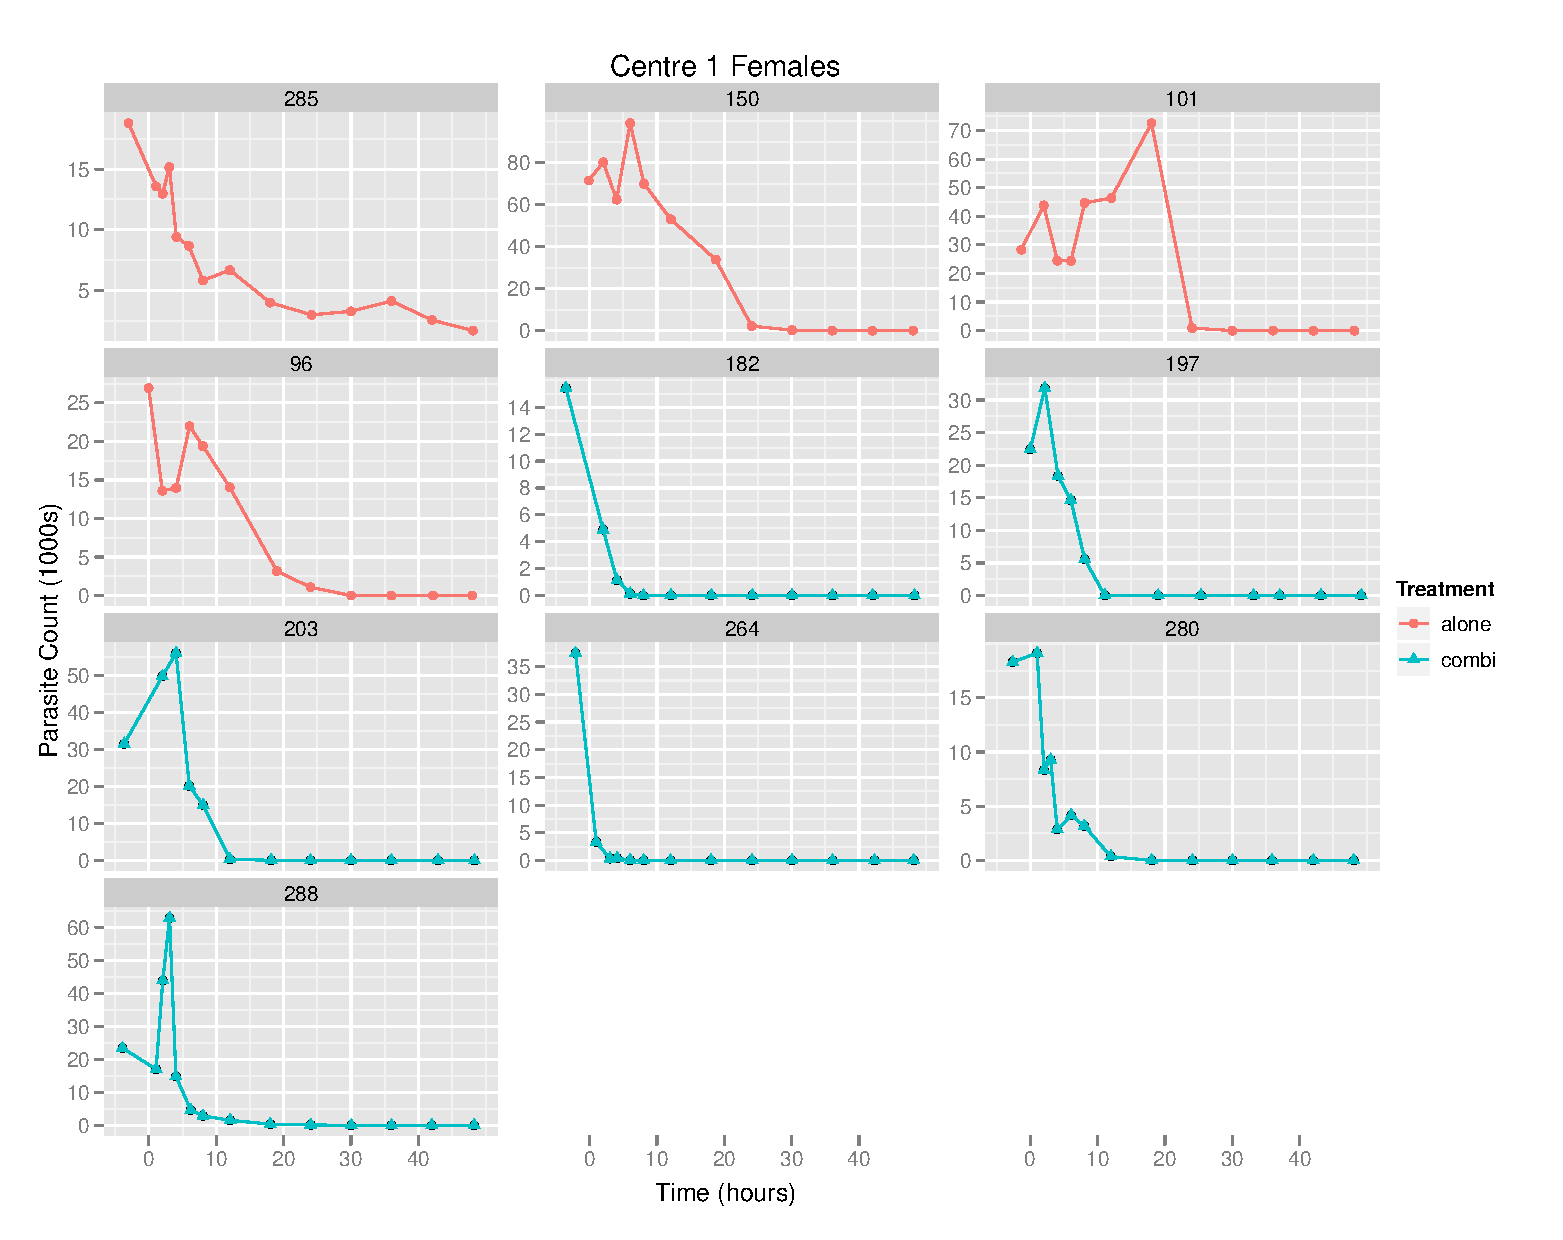
\includegraphics[width=6.1in]{raw1f.eps}
\caption{Parasite count for centre 1 females}\label{raw1F}
\end{figure} 
\begin{figure}[h]
\centering
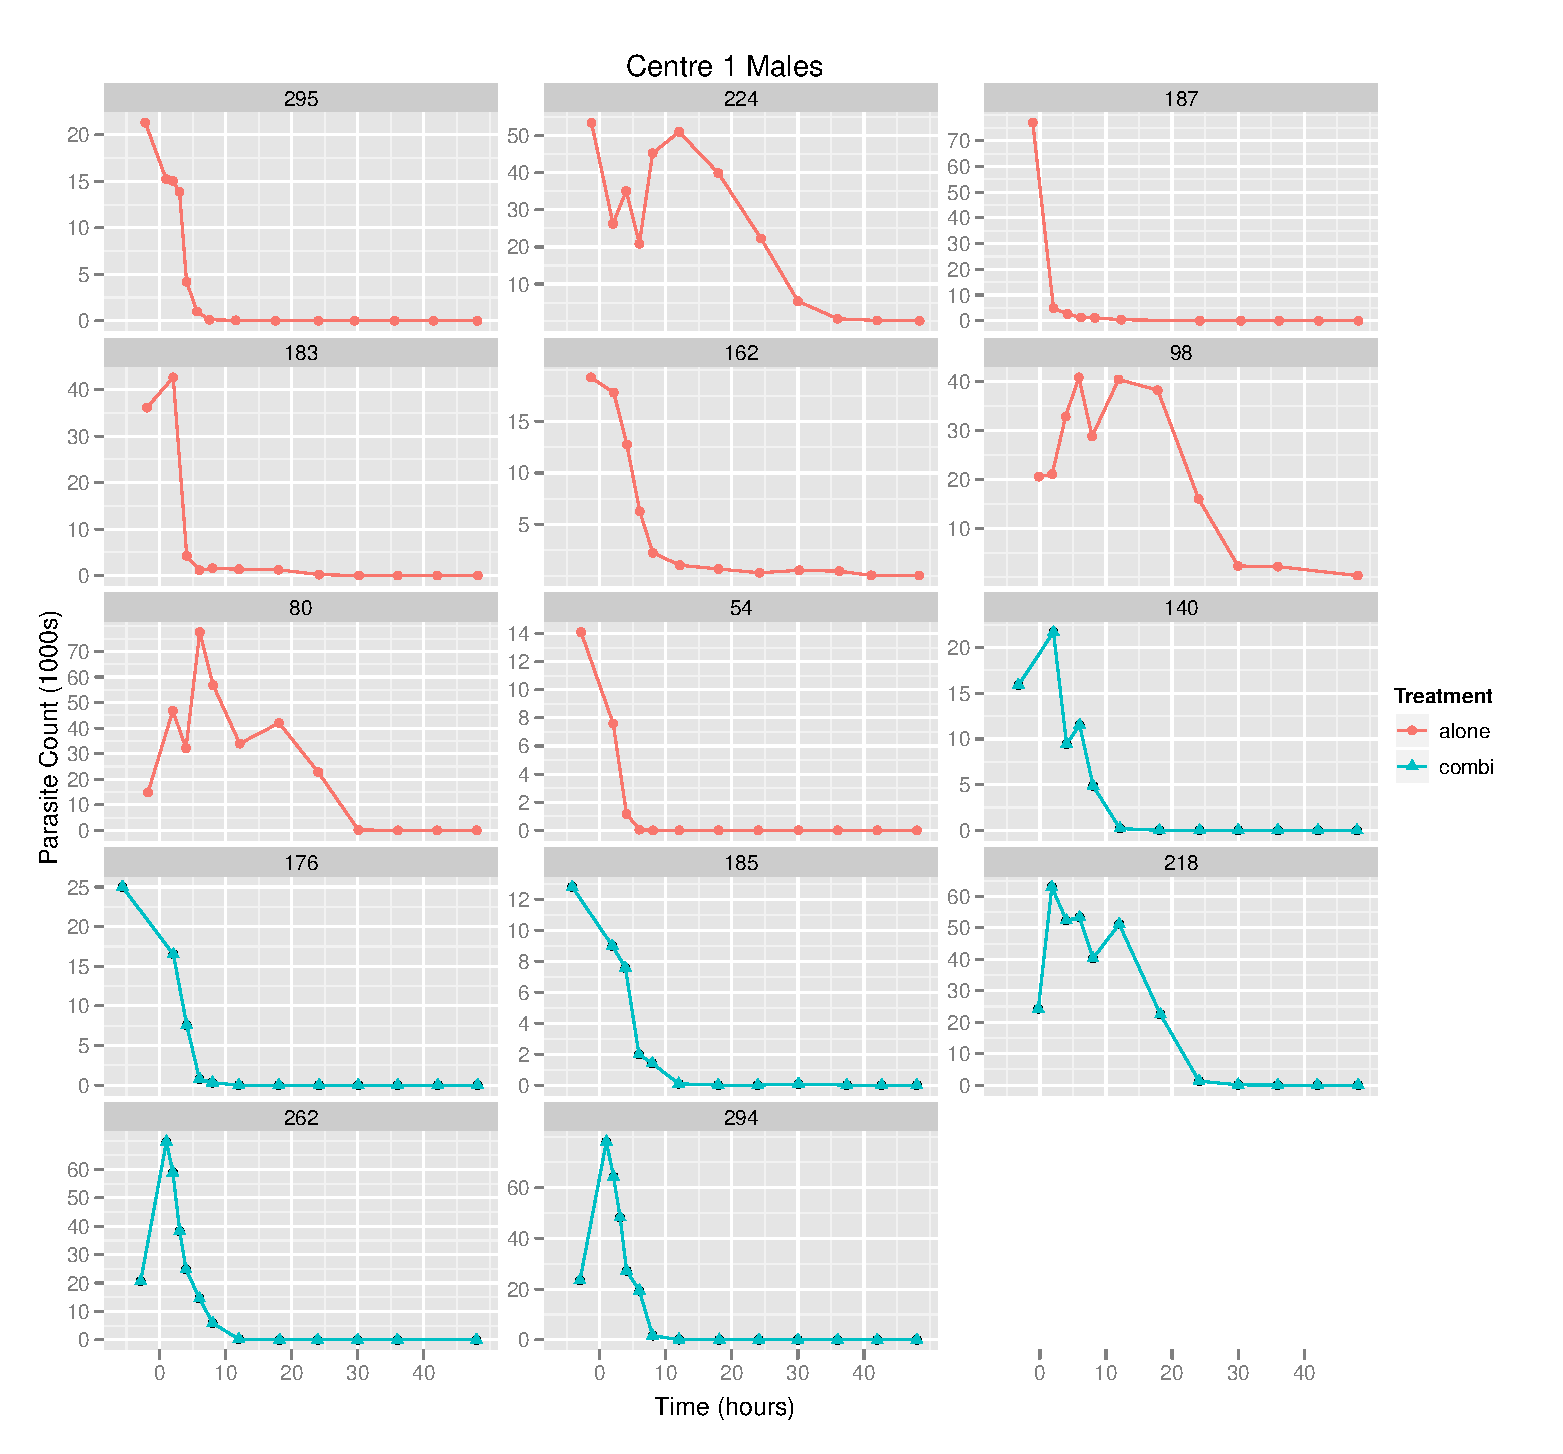
\includegraphics[width=6.1in]{raw1m.eps}
\caption{Parasite count for centre 1 males}\label{raw1M}
\end{figure} 
\begin{figure}[h]
\centering
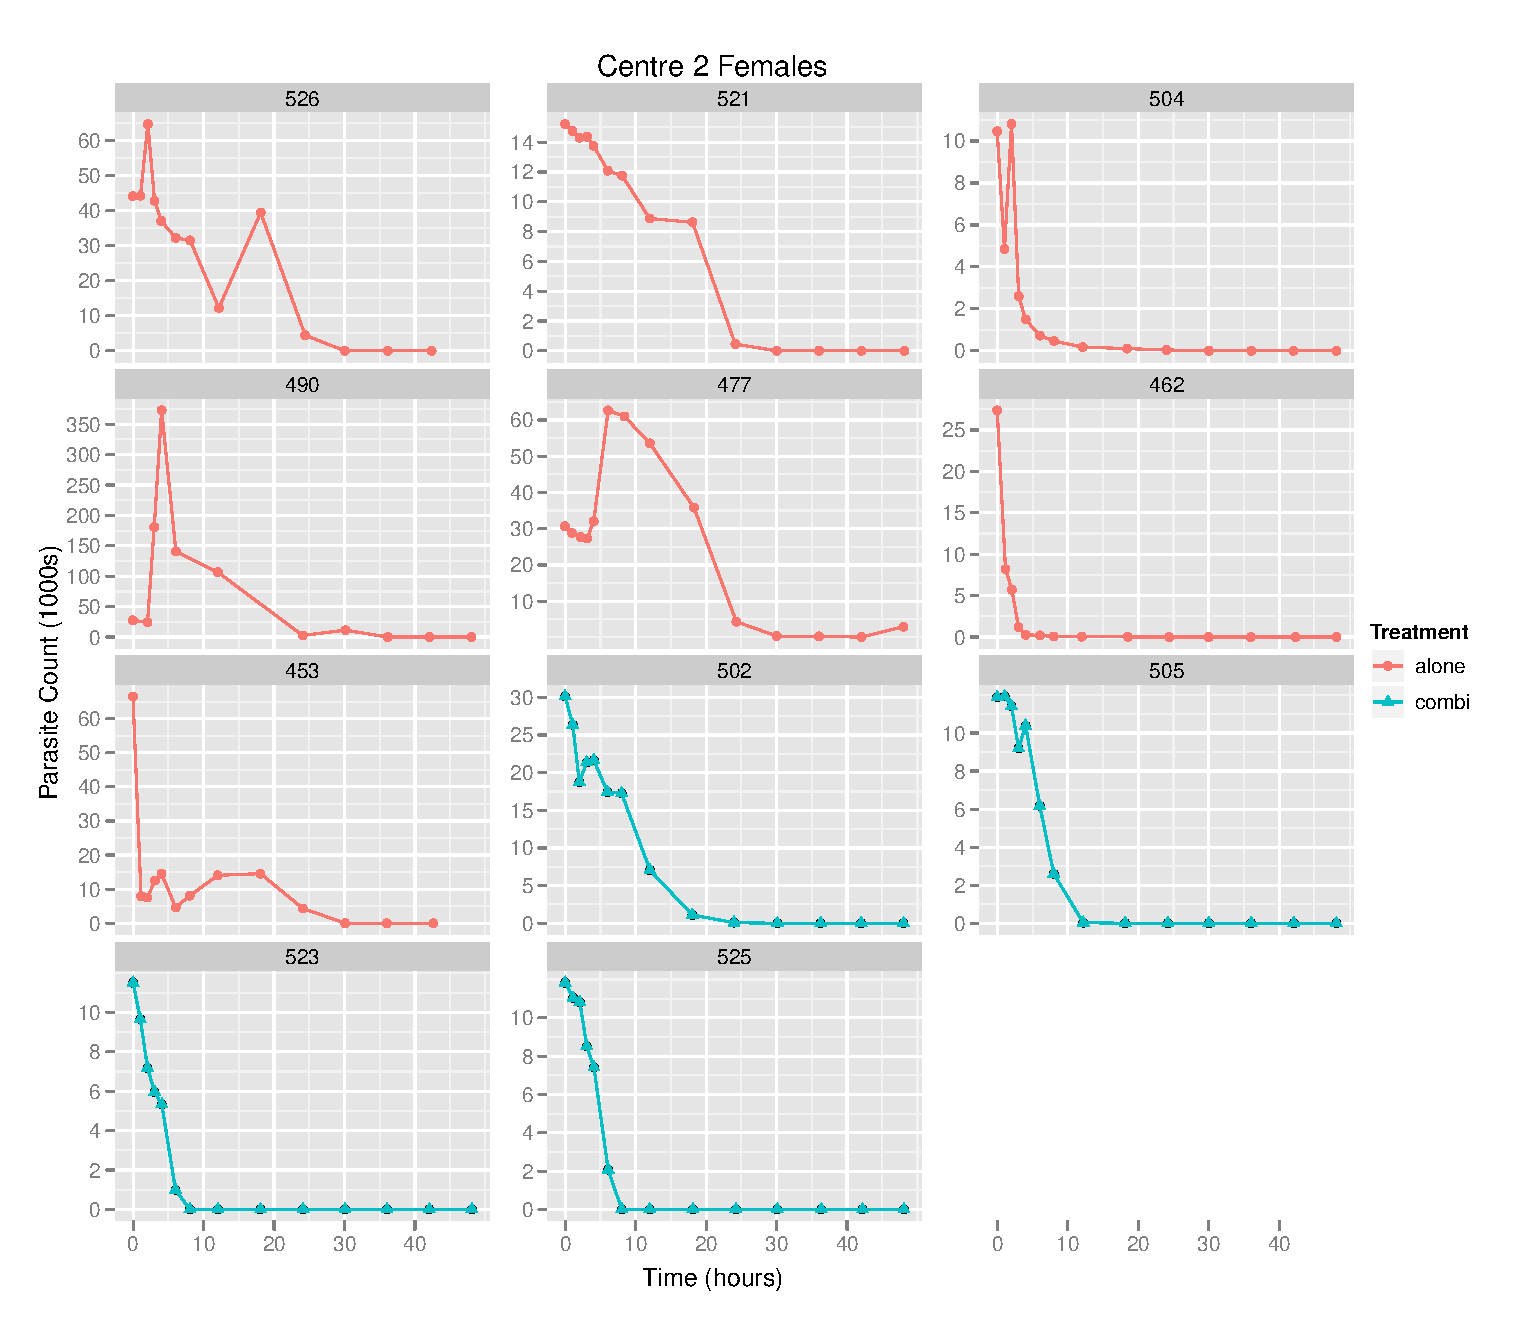
\includegraphics[width=6.1in]{raw2f.eps}
\caption{Parasite count for centre 2 females}\label{raw2F}
\end{figure} 
\begin{figure}[h]
\centering
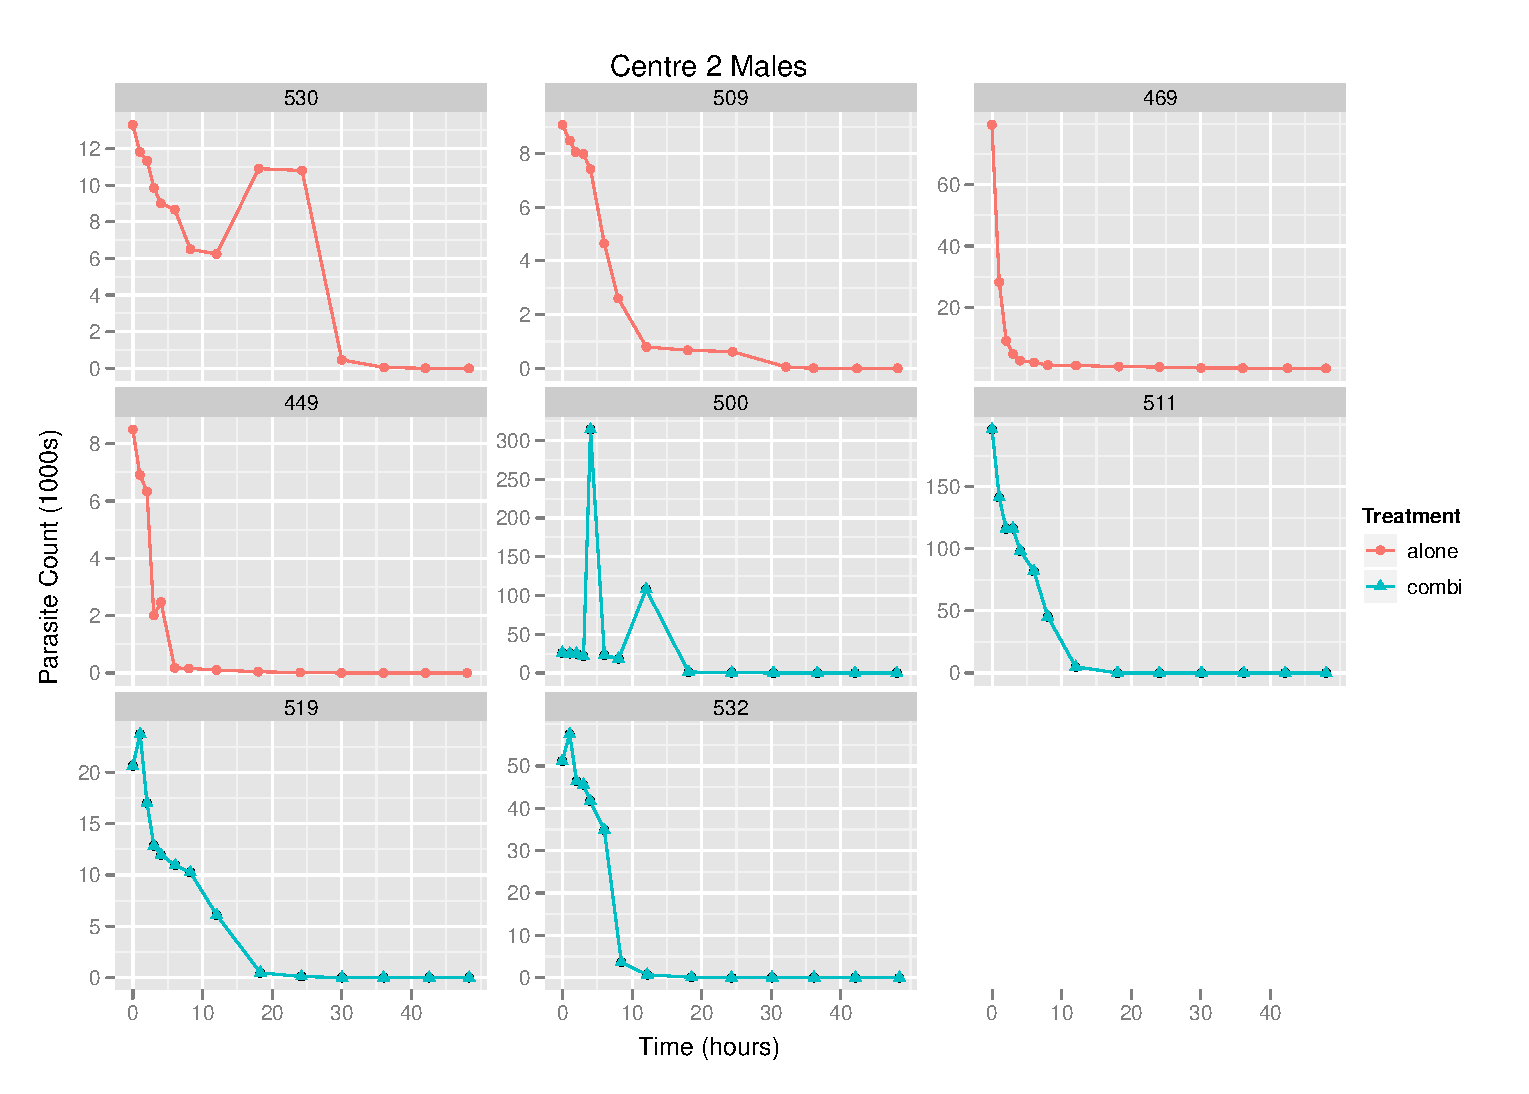
\includegraphics[width=6.1in]{raw2m.eps}
\caption{Parasite count for centre 2 males}\label{raw2M}
\end{figure} 
\subsection{Main features of the data}
Generally, there appears to be a drop in the parasite count from an initial high level to zero or near zero within about 20 to 30 hours from first treatment. In some cases there is a rapid monotonic drop off within 10 hours. In other cases the \textit{recorded} parasite count fluctuates up and down before dropping to zero over a longer period.

To briefly summarise, the main behaviours observed are:
\begin{itemize}
\item A relatively steep monotonic drop in the count e.g. centre 1 female subjects 182 and 264 (Figure \ref{raw1F}), centre 1 male subjects 187, 162, 54, 176 and 185 (Figure \ref{raw1M}), centre 2 female subjects 462, 523 and 525 (Figure \ref{raw2F}) and centre 2 male subjects 509, 469 and 511 (Figure \ref{raw2M}).

A variation of this type has the parasite count increasing after the first dose before falling e.g. subjects 197 and 203 (Figure \ref{raw1F}) and subjects 262 and 294 (Figure \ref{raw1M}). White\cite{white} notes that ``\textit{parasitemia may rise alarmingly in the hours following treatment}'' and gives reasons therein.
\item A more erratic and slower drop in the parasite count e.g. centre 1 female subjects 285 and 96 (Figure \ref{raw1F}), centre 1 male subjects 295 and 140 (Figure \ref{raw1M}) and centre 2 female subjects 521, 502 and 505 (Figure \ref{raw2F}). 
\item The parasite count seems to fluctuate about a constant level before falling e.g. centre 1 female subjects 150 and 101 (Figure \ref{raw1F}) and centre 1 male subjects 224, 98, 80 and 218 (Figure \ref{raw1M}). 
\end{itemize}
There are some profiles that we might suspect contain anomalous data such as subject 500 in Figure \ref{raw2M} where there are two unusually high values compared to the main trend. We might suspect that some inconsistency in the counting procedure explains this behaviour rather than the patient's parasite count jumping by a large amount on these occasions. Looking at how the parasite count was obtained should give an insight into potential sources of inconsistency.
\subsection{Implications for modeling}
It can be seen from the parasite count profiles in Figures \ref{raw1F} to \ref{raw2M} that no simple linear model will closely approximate the behaviour of all patients' counts over the whole time range. However, as we are primarily interested in estimating the time to reduction of the parasite count by 90\% it is only really in this region that it is critical to find a good model. It may be that the erratic behaviour of some parasite counts at short times after first dose is of little relevance. With this in mind, one possible approach may be to use a logarithmic transform of the parasite count thereby emphasising the behaviour at low counts.
\section{Properties of the Parasite Count}
\subsection{Derivation of the Parasite Count}
One of the first questions addressed was whether the parasite count is a true count, and thus Poission statistics would be applicable, or whether it is a derived measurement. Our contact informed us that the method used to arrive at the parasite count values given is broadly as follows.
\begin{enumerate}
 \item A microscopist would choose ``suitable area'' of a slide of blood and work from left to right counting parasites ($N_p$) and white blood cells ($N_w$).
\item If by the time they have counted around 200 white blood cells they have seen less than 10 parasites then they continue counting until they have counted around 500 white blood cells.
\item The number of white blood cells in a $\mu L$ of blood ($\rho_w$) is automatically counted by a machine.
\end{enumerate}
Accordingly the number of parasites in a $\mu L$ of blood (\texttt{parct}) is given by:
$$\mathtt{parct}=\frac{N_p}{N_w}\rho_w$$
and thus we cannot treat this derived measurement as a count for modeling purposes.
\subsection{The Pre-dose parasite count}
We were also informed that the white blood cell count is right skewed and so we might expect that the parasite count per $\mu L$ will be also.
%Table \ref{predose} shows the pre-treatment parasite counts in the subjects from each test centre and of each sex. It can be seen that for 3 cases the mean is larger than the median meaning that the distributions are right skewed. This is to be expected for non-negative data such as this. When model fitting to this data we may have to choose some transformation of the parasite count such as taking logarithms.
Figure \ref{preaov} shows the pre-dose parasite counts grouped by sex, centre and treatment. There does not seem to be an obvious dependence of the level of the pre-dose parasite count on sex, centre or treatment.
\begin{figure}[h]
\begin{center}
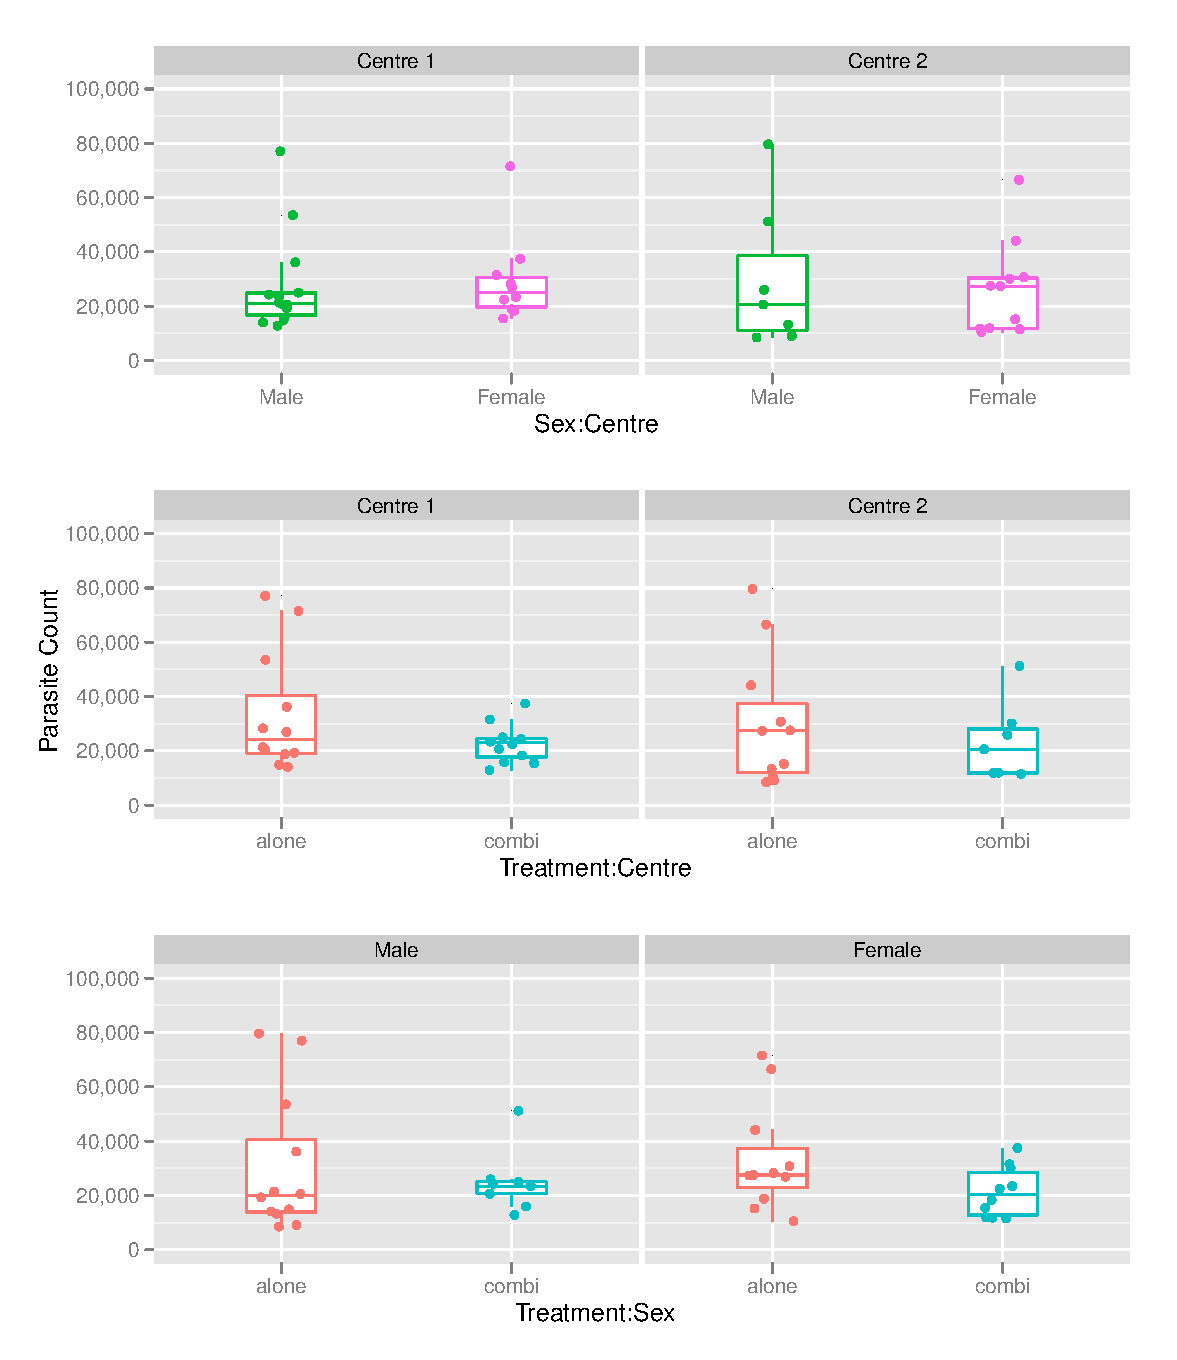
\includegraphics[width=6.1in]{preaov.eps}
\caption{Pre-dose parasite counts by sex, centre and treatment with mean shown. The right-hand column of panels shows both sexes combined grouped by centre; the bottom row shows both centres combined, grouped by sex and the bottom-right corner panel shows both sexes and centres combined.}
\label{preaov}
\end{center}
\end{figure}

If we perform 3-way ANOVA of the pre-dose parasite count by sex, centre and treatment we find that there is no evidence of a dependence on these factors. The Kruskal-Wallis non-parametric equivalent test also does not reveal any evidence of a dependence.

Figure \ref{aovres} shows that the residuals from the ANOVA are right-skewed. If we repeat the ANOVA but with the logarithm of the pre-dose parasite count we find that the residuals are approximately normally distributed as shown in Figure \ref{logaovres}. Using the square-root of the count does not produce as good a normalising transformation: Shapiro-Wilk normality test returns $P<0.0001$ compared to $0.1<P<0.05$ for the logarithmic transformation. 
\begin{figure}[p]
\begin{center}
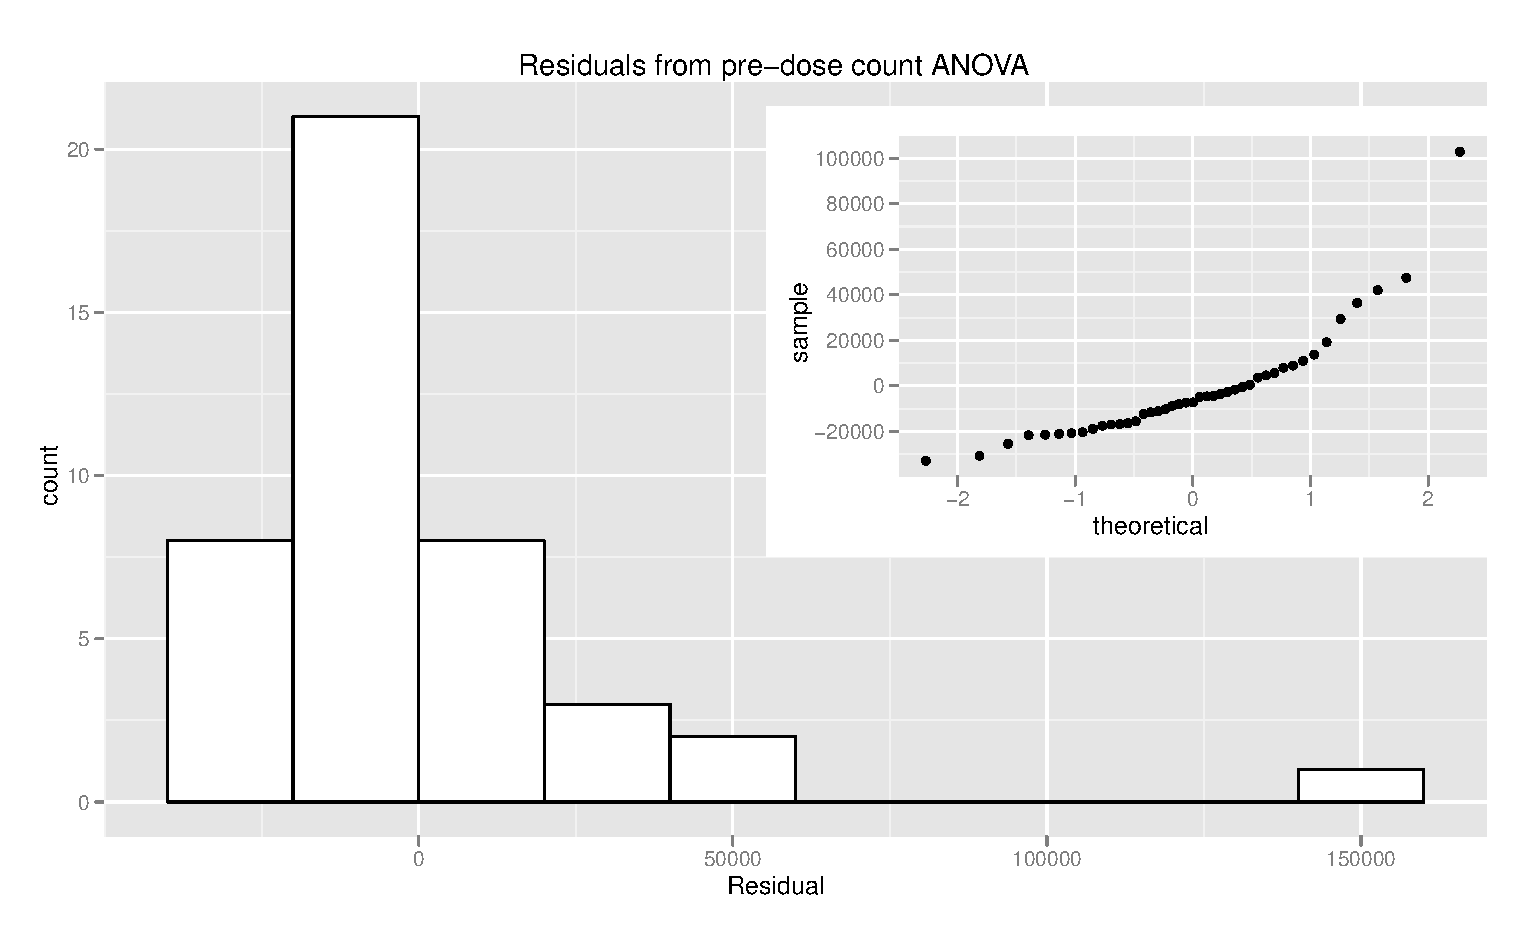
\includegraphics[width=6.1in]{aovres.eps}
\end{center}
\caption{Residuals from 3-way ANOVA of pre-dose parasite counts}
\label{aovres}
\end{figure} 
\begin{figure}[p]
\begin{center}
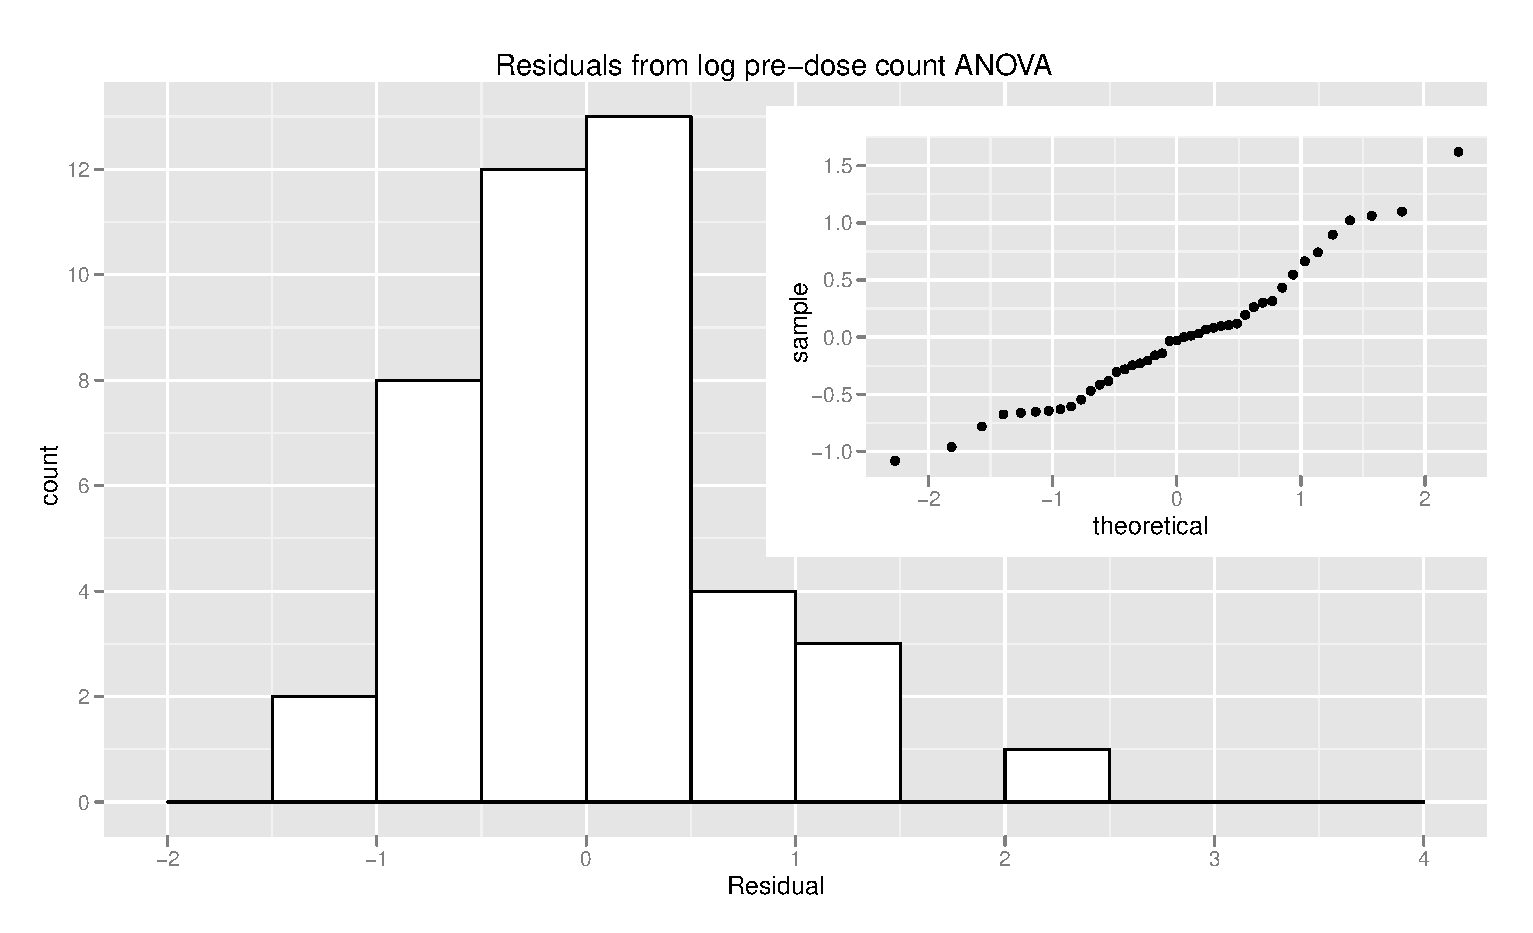
\includegraphics[width=6.1in]{logaovres.eps}
\end{center}
\caption{Residuals from 3-way ANOVA of log pre-dose parasite counts}
\label{logaovres}
\end{figure} 
% \begin{table}[h]
% \centering
% \caption{Pre-dose parasite counts}\label{predose}
% \begin{tabular}{|cc|cccccc|}
% \hline
% Centre&Sex&N&Mean&Median&SD&1st Qu.&3rd Qu.\\\hline
% \multirow{2}{*}{001}&M&14&27060&20960&17820.9&16750&24830\\
% &F&10&29410&25170&16221.2&19700&30700\\\hline
% \multirow{3}{*}{002}&M&8&50540&23290&63679.9&12240&58290\\
% %&$M^*$&\textit{7}&\textit{29750}&\textit{20610}&\textit{26436.6}&\textit{11180}&\textit{38580}\\
% &F&11&26110&27360&17262.4&11860&30400\\\hline
% \end{tabular}
% \end{table}
\section{Development of the parasite count with time}
Figure \ref{allaov} shows the progression of the parasite count for all patients with time from first dose, grouped by sex, centre and treatment, with the ``marginal plots'' in the right column and bottom row as before. The vertical axis is the logarithm of the fraction of the pre-dose parasite count:
$$y=log\left(\frac{1+P_t}{P_0}\right)$$
where $t$ is the time from first dose and $P_0$ is the pre-dose count. $1+P_t$ is used to avoid problems with taking the logarithm when the parasite count goes to 0.

With regard to Figure \ref{allaov}, the behaviour as indicated by the average response lines can be summarised as follows:
\begin{itemize}
 \item For female patients on the single-drug (``alone'') treatment the parasite count remains close to the initial level up to about 20 hours from first dose before beginning to fall off.
 \item For male patients on the single-drug treatment the parasite count falls off at a fairly constant rate from first dose, perhaps increasing in fall-off rate after 20 hours.
\item There doesn't seem to be as remarkable a difference between male and female subjects on the combined-drug treatment with parasite counts starting to show an appreciable fall off after about 5 hours in both cases.
\item There is not a readily noticeable difference between centres.
\end{itemize}
In summary it appears from this first rough comparison that the combined treatment is more effective in terms of clearance times than the single treatment. This improvement over the single treatment seems more marked for female patients, but primarily because the single treatment seems to be less effective for female patients with the combined treatment fall-off profile being similar for both sexes.
\begin{sidewaysfigure}[p]
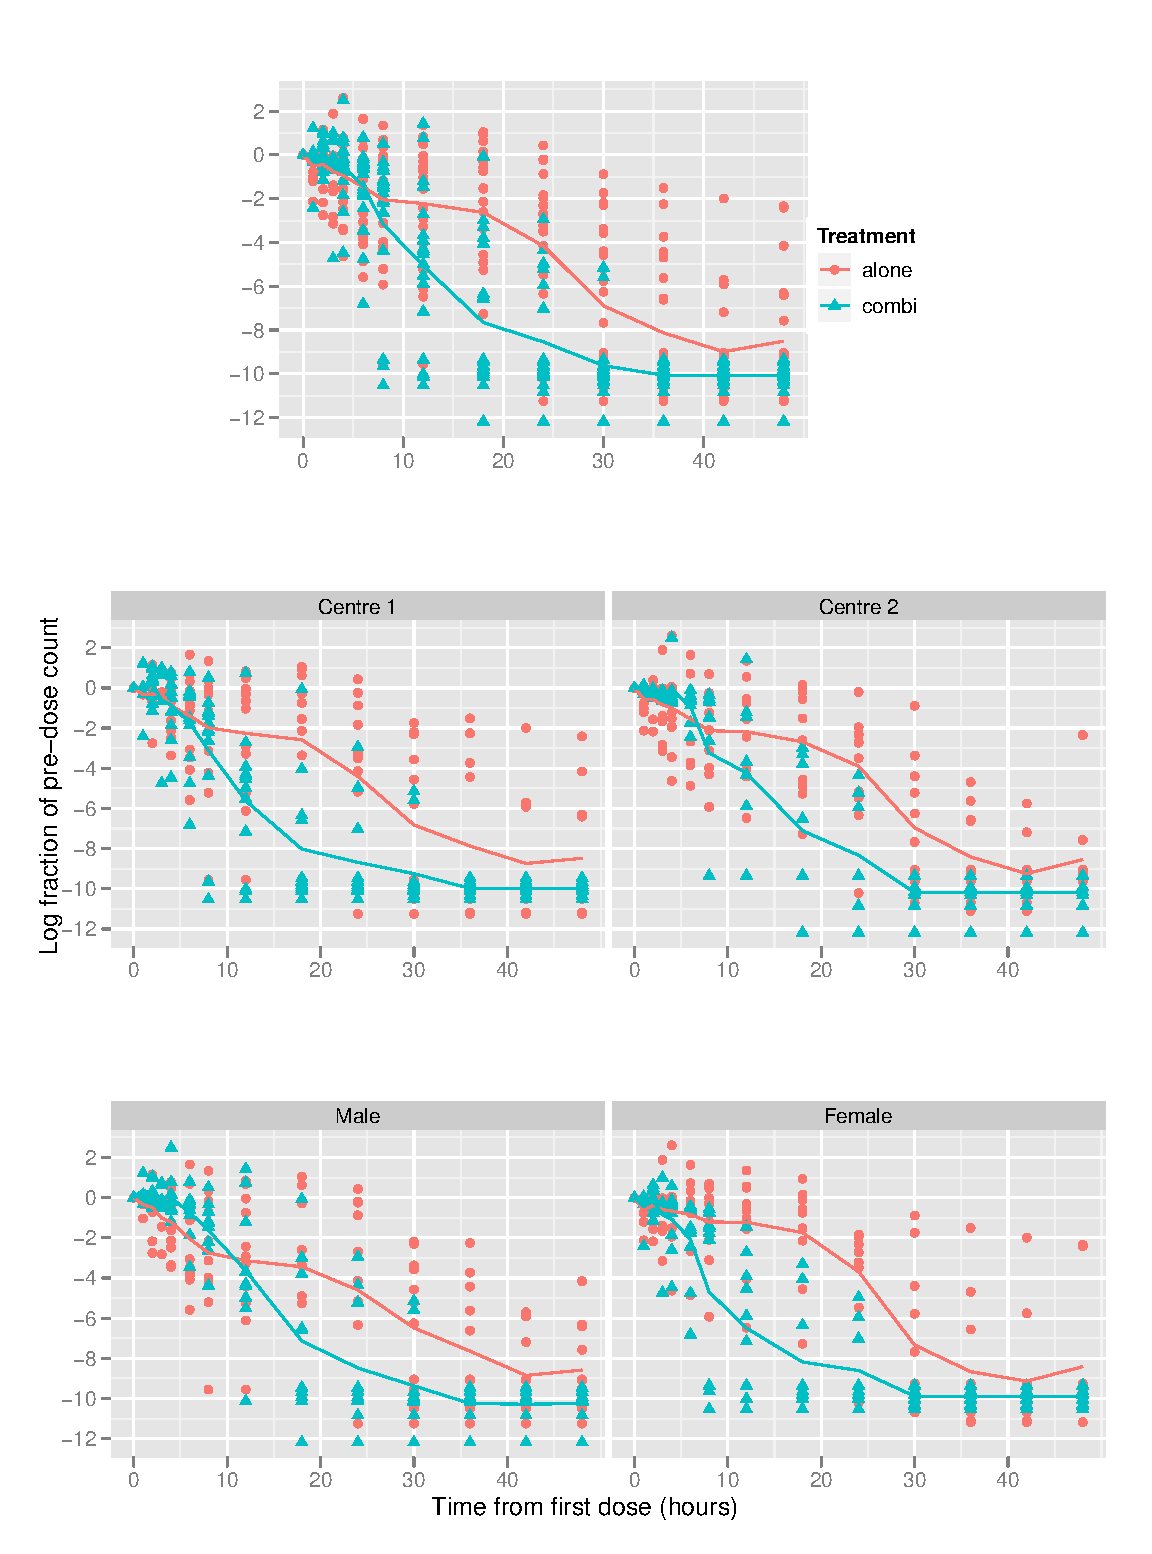
\includegraphics[width=9.2in]{allaov.eps}
\caption{Parasite count as proportion of pre-dose count with time from first dose with mean levels shown}
\label{allaov}
\end{sidewaysfigure}

If we repeat the 3-way ANOVA as for the pre-dose counts but with the logarithm of the counts at 6, 12, 18 an 24 hours from first dose then we find strong evidence of a dependence of the count on the treatment, which can be seen graphically in the bottom-right panel of Figure \ref{allaov}. We also find at 6 and 12 hours evidence of an interaction between sex and treatment, $P<0.05$ and $P<0.01$ respectively, bearing in mind we are making multiple hypothesis tests and therefore should be more hesitant to draw any early conclusions. At 18 and 24 hours there is no evidence of an interaction with sex, only a treatment effect $P<0.0001$. We can attempt to get some insight into the interaction of sex and treatment effects by looking at the bottom-left and bottom-centre panels of Figure \ref{allaov}, although it is not easily interpretable at this stage, if there is a substantial interaction at all.

The residuals from all these ANOVA analyses are normally distributed to a good approximation. This is not so if we use the counts without taking logarithms in all cases.
\section{Key findings}
Our initial findings after exploratory graphical and preliminary ANOVA analyses are:
\begin{itemize}
\item The parasite data appears to be right-skewed and a logarithmic transformation seems to be appropriate to remedy this. Wootton \textit{et al.}\cite{wootton} chose a logarithmic transformation of the parasite count in their study of similar data.
\item The pre-dose parasite count does not seem to be related to sex, centre or intended treatment.
\item The parasite count after treatment shows dependence on the treatment with possibly some interaction with the sex of the subject.
\end{itemize}

In the next chapter we will go on to look at how to estimate the endpoint of primary importance for subjects, the time to reduce the parasite count by 90\%.